"TSF consists of multiple trees and is difficult to understand", so 
there is need for a method to extract interpretability from a 
forest. The temporal importance curve is introduced to reveal which parts of the 
time series contribute most to the classification decision. For that am importance function is built for each feature type and
used for all time points of the dataset. The Curve then is built by graphing those results out.

The importance function is based on the entropy gain of each split node $v$ in the forest $SN$ for the given feature type. All the 
nodes which intervals time-point $t$ are considered and their entropy gain for the given feature type is 
summed up. If the feature is not used in the split of the node, the entropy gain is set to zero.

\[
	\operatorname{Imp}_k(t) = \sum_{t_{start} \leq t \leq t_{end}, v \in SN}
\]

The method reveals temporal patterns in the data relevant for classification. Peaks in the curve indicate time regions used by strong splits.
Because points in the center of the series appear in more intervals, there is a natural bias towards them. To counteract this, the authors compare
uninformative datasets with the calculated importance curve (\Cref{fig:tempOne}).

In practice, the curves highlight discriminative intervals successfully (\Cref{fig:tempTwo}).
As an example, the temporal importance curves peak precisely in regions with specific intervals between the classes (\Cref{fig:tempTwo}).

Using this method of observing the strength of the splits, it can be shown that entrance gain gives sharper and 
more localized peaks, thus improving the interpretability and specificity of the importance curves.

\begin{figure}[h]
\centering
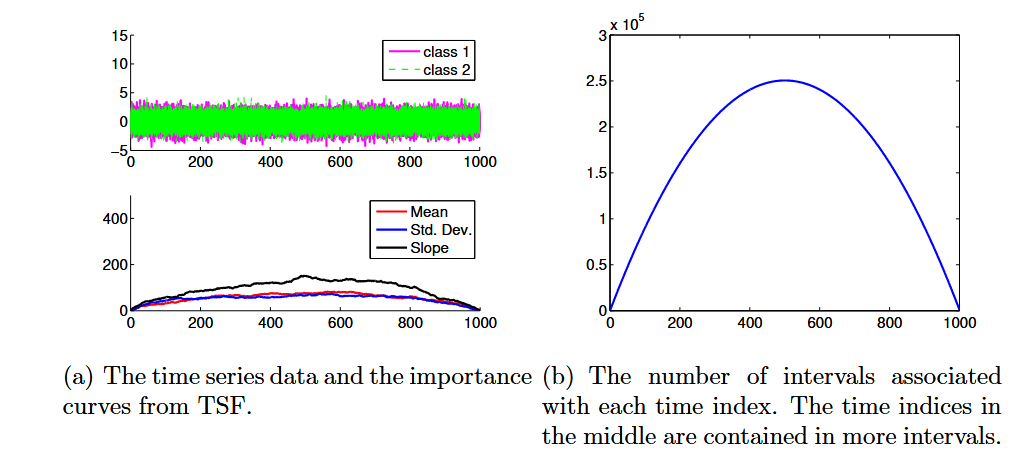
\includegraphics[width=\linewidth]{res/importanceCurvesOne.png}
\caption{When no feature is important for classification, the curves have larger values in the center due to more interval overlap.}
\label{fig:tempOne}
\end{figure}

\begin{figure}[h]
\centering
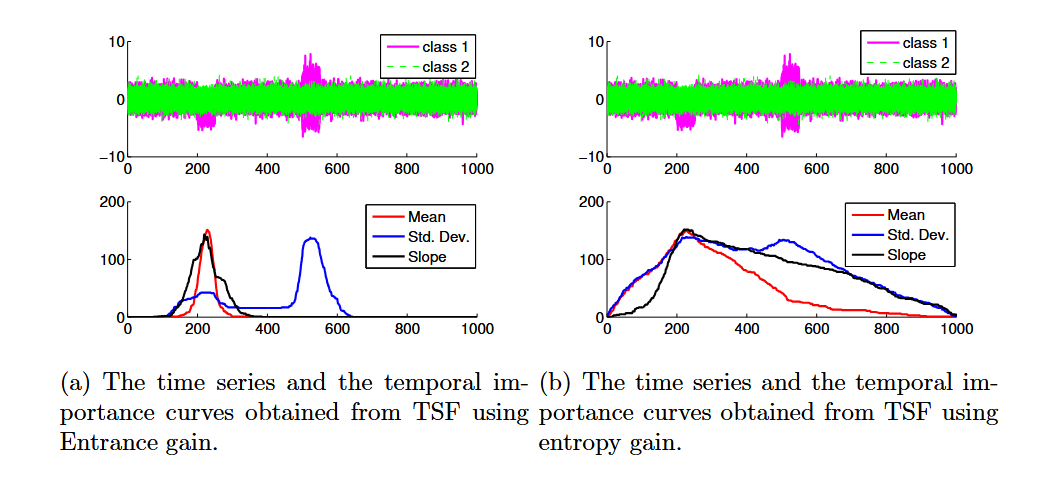
\includegraphics[width=\linewidth]{res/importanceCurvesTwo.png}
\caption{The time series from two classes differ in mean and standard deviation at specific intervals. Entrance gain curves show sharper, localized peaks.}
\label{fig:tempTwo}
\end{figure}
